
\section{PyPV: An easy Current-Voltage curves acquisition interface}

	\epigraph{\textit{"Ok, I finally completed it, by the way, why did you start developing this?"\\"Well, it was just a proof of concept, but it's nice you worked on it"}}


	\subsection{Previous software}
		\begin{SCfigure}%[!hbtp]%
			\centering
			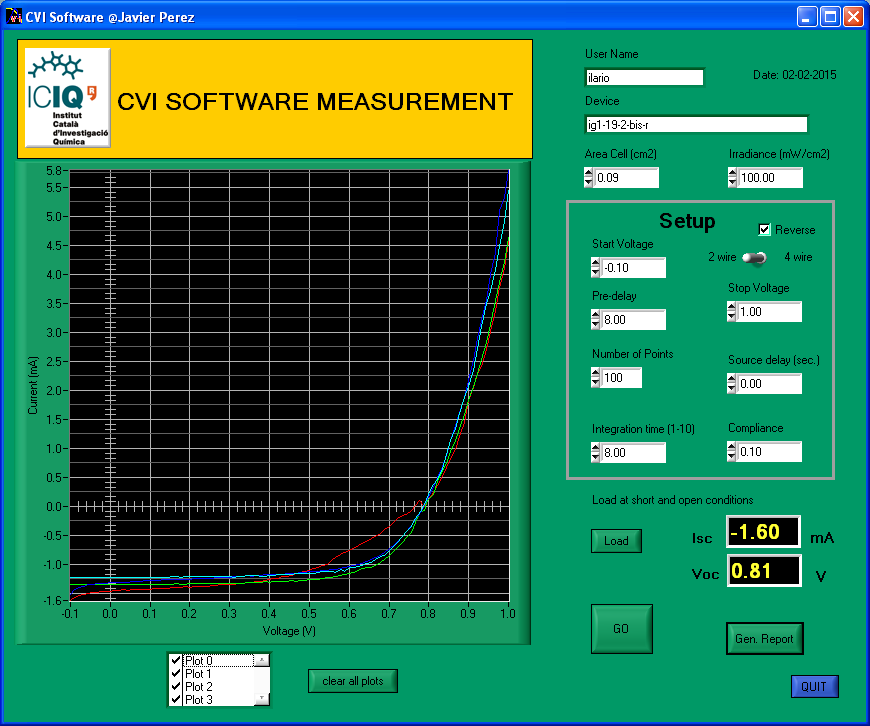
\includegraphics[width=0.5\textwidth]{old_iv_software/old_iv_software.png}
			\caption{}\label{fig:old_iv_software}
		\end{SCfigure}

	\subsection{Original Project}
		I received a proof-of-concept software developed by Daniel Fernandez Pinto and decided to continue the development. At that point the software had an interface with few buttons and a working Keithley communication library.

	\subsection{User's requests}

		Installation instructions
		Shutter control
		GPIB GPIB0
	\subsection{Implementation and user interface}

		\paragraph{Autoscale} As it was explained in \cpageref{autoscale}, the automatic scale setting of the Keithley is detrimental for perovskite solar cells dynamic measurements.

		\paragraph{Auto-measure}\label{automeasure}

		\paragraph{Resistances} The shunt and series resistances estimation from current-voltage sweeps have been implemented but should not be considered for measurements on hysteretic devices, as explained in \cpageref{resistances}.
		
		\paragraph{Scan speed calculation} 
		The scan speed $s[V/s]$ is obtained from the voltage step \texttt{:SENSe:VOLTage:STEP} $V_|step|[V]$, integration time \texttt{:SENSe:VOLTage:NPLCycles} $n_|int|$ measured in power line cycles and the delay time \texttt{:SOURce:DELay} $t_|delay|[s]$ Keithley's parameters with the following \textit{empirical} expression:
		
		\begin{equation}
		s = \frac{V_|step|}{0.003 + t_|delay| + 0.06 \cdot n_|int|}
		\end{equation}
		
		where $t_|delay|$ is \SI{1}{\ms} for our measurement conditions \cite{Keithley2011}.

	\subsection{Limitations}

		The interface development has been started with the "Monkey Studio" software, which development has ceased even before the start of PyPV. This demonstrated to be a big failure in long term development planning.

\section{Robust and quick data analysis \textit{via} R scripts}
	\epigraph{\textit{"Is there an Origin version for Linux?"\\"No"}}


	\subsection{Charge Extraction (\glsentryshort{ce})}\label{r_ce}


	\subsection{Transient PhotoVoltage (\glsentryshort{tpv})}\label{r_tpv}

	\subsection{Transient PhotoCurrent (\glsentryshort{tpc})}\label{r_tpc}

	\subsection{Differential Capacitance (\glsentryshort{dc})}\label{r_dc}

\section{Maximum Power Point Tracking}\label{software_mppt}
	\epigraph{\textit{"A student of mine sells a complete system for that, just go and buy it"}}

	\cite{Cimaroli2017,CandlelightSystems}
